\section{Introduction}

\subsection{Antibiotic resistance}

Antibiotics add, on average, twenty years to a person's life\cite{davies2013drugs}. However, antibiotic resistance is increasing alarmingly and is now recognised as a major threat to global health\cite{ResistanceUS,davies2013drugs}. Antibiotic discovery had its heyday in the 1940s to 60s, which saw the discovery of many new classes of antibiotic. Since then, the rate of discovery of new classes has slowed and resistance to existing treatments has increased.

The story of how Alexander Fleming discovered penicillin by accidentally allowing a Petri dish containing \textit{Staphylococcus aureus} to become contaminated with \textit{Penicillium} mould whilst he was on holiday in Suffolk \cite{davies2013drugs} is well known to many scientists. The initial serendipitous discovery of penicillin occurred in 1928 and was reported in 1929\cite{Fleming1929}, but it was not until 1943 that the drug was mass produced thanks to the research of Ernst Chain and Howard Florey. However, bacterial resistance to penicillin was being found in hospitals by the late 1940s \cite{Barber1947, Rountree1949}. This alarmingly quick emergence of resistance is a common phenomenon for antibiotics (see \ref{tbl:AB_timeline}) as bacteria have multiple resistance mechanisms against antibacterial agents. These mechanisms can be broken down into five main categories:

\begin{enumerate}
\item The bacterium may inactivate the drug before it can cause damage, for example the hydrolysis of $\beta$-lactam antibiotics such as penicillin by $\beta$-lactamase enzymes.

\item The bacterium may produce a membrane, cell wall or biofilm which does not allow the drug to pass through, for example biofilm formation may allow bacterial resistance to antibiotics to increase 1000-fold compared with bacteria in suspension culture\cite{Stewart2001}.

\item The bacterium may pump antibacterial molecules out of its cell membrane using efflux pumps, for example the mexAB and mexXY pumps used by \textit{Pseudomonas aeruginosa}\cite{Poole2004}.

\item Mutations may cause the target of the antibacterial molecule to alter such that the molecule no longer effectively binds the target, for example the alteration of penicillin binding proteins which are involved in the final stages of peptidoglycan biosynthesis in the cell walls of MRSA and other penicillin-resistant bacteria\cite{Fuda2004}.

\item The bacterium may switch to using a metabolic pathway which does not involve the target of the antibacterial molecule, for example sulfonamide resistance may be achieved by taking in folic acid from the environment rather than synthesising it using \textit{p}-aminobenzoic acid - a process which is blocked by sulfonamides\cite{Skold2000}.

\end{enumerate}

\begin{table}[H]
  \centering
\begin{tabular}{|p{0.15\textwidth}|p{0.13\textwidth}|p{0.11\textwidth}|}
\hline  
\textbf{Antibiotic} & \textbf{Introduction} & \textbf{Resistance} \\ 
\hline
Sulfonamides & 1930s & 1940s \\ 
\hline 
Penicillin & 1943 & 1946 \\ 
\hline 
Streptomycin & 1943 & 1959 \\ 
\hline 
Chloramphenicol & 1947 & 1959 \\ 
\hline 
Tetracycline & 1948 & 1953 \\ 
\hline 
Erythromycin & 1952 & 1988 \\ 
\hline 
Vancomycin & 1956 & 1988 \\ 
\hline 
Methicillin & 1960 & 1961 \\ 
\hline 
Ampicillin & 1961 & 1973 \\ 
\hline 
Trimethoprim & 1962 & 1972 \\
\hline 
Cephalosporins & 1960s & late 1960s \\
\hline 
Ciprofloxacin & 1987 & 1988 \\
\hline 
Linezolid & 2000 & 1997 \\
\hline
Daptomycin & 2003 & 2005\\
\hline
\end{tabular}
\caption{A timeline of when various antibiotics were first introduced and when resistance to them first appeared\cite{Clatworthy2007,Palumbi2001,Ogle1988,Huovinen2001,Birmingham2003,Lee2007}.\label{tbl:AB_timeline}} 
\end{table}


\subsection{Quorum sensing}

A quorum is defined as `A fixed minimum number of members of an assembly or society that must be present at any of its meetings to make the proceedings of that meeting valid.' \cite{Dictionary}  
A similar concept is used in bacterial signalling, whereby group behaviour is only triggered when a certain minimum population of bacteria has been reached. Examples of group behaviour include bioluminescence, the  production of  virulence factors and biofilm formation.  
It is advantageous for bacteria to coordinate such behaviours as they would be ineffective, and therefore a waste of resources, when carried out by a single bacterium but effective when carried out as a group.

\subsubsection{\textit{Vibrio fischeri}}

The first example of quorum sensing was discovered in \textit{Vibrio fischeri}, a symbiotic bacterium that produces bioluminescence in the photophore of the Hawaiian bobtail squid, \textit{Euprymna scolopes} \cite{Nealson1970a,Miller2001,Visick2006} (see \ref{fig:ES+MJ}a). This bacterium receives amino acids\cite{Graf1998, Lemus2000} from its host in exchange for producing light which the squid uses for counterillumination, to camouflage itself\cite{Jones2004} (\textit{V. fischeri} also has symbiotic relationships with other species, including the Japanese pinecone fish, \textit{Monocentris japonica}\cite{Ruby1976})(see \ref{fig:ES+MJ}b). 

\begin{figure}[H]
	\begin{center}
		\begin{tabular}{cc}
	    	\textbf{a} & \textbf{b}\\
			\includegraphics[width=0.45\textwidth, height=5cm]{Euprymna_scolopes.jpg} & \includegraphics[width=0.45\textwidth, height=5cm]{Monocentris_japonica.jpg} \\
			
		\end{tabular}	
		
		\caption{a) "Euprymna scolopes, South shore of Oahu, Hawaii" by Jamie Foster. Licensed under CC BY-SA 3.0 via Commons. 
		b) "Monocentris japonica.1 - Aquarium Finisterrae" by Drow\texttt{\_}male. Licensed under GFDL via Commons. \label{fig:ES+MJ}}
		
	\end{center}
\end{figure}


If a low population  of \textit{V. fischeri} is  present  in  the  photophore,  the  light  that the bacteria could produce would  be insufficient to  attract prey. Therefore, the bacteria conserve resources by not producing light.
However, if there is a high population of \textit{V. fischeri} it is useful for them all to produce light, as this incentivises the squid to provide them with nutrients. 

\subsubsubsection{The LuxR-LuxI system}

The bacteria sense the population of other \textit{V. fischeri} in their vicinity by the detection of 3-oxo-C$_6$-HSL \compound{cmpd:HLO6}\cite{Eberhard1981} (see \ref{fig:HLO6}), a freely diffusible\cite{Kaplan1985} molecule which is secreted by all \textit{V. fischeri} cells\cite{Schaefer1996} at a low basal level\cite{Miller2001}. When the bacterial population density, and hence the concentration of 3-oxo-C$_6$-HSL \compound{cmpd:HLO6}, reaches a threshold, a response is triggered leading to expression of high levels of luciferase, and hence a 10,000-fold\cite{Devine1989} increase in the production of (blue-green%\cite{Greenberg1999}) light\cite{Engebrecht1983}. A positive feedback mechanism leads to further production of 3-oxo-C$_6$-HSL \compound{cmpd:HLO6} and hence amplification of the signal. This is the reason that 3-oxo-C$_6$-HSL \compound{cmpd:HLO6} is known as an autoinducer.

The quorum sensing system of \textit{V. fischeri} consists of two operons (see \ref{fig:VF_QS}). The left operon encodes just one gene, \textit{luxR}, a transcription factor which binds 3-oxo-C$_6$-HSL \compound{cmpd:HLO6}. The right operon encodes \textit{luxICDABEG}. \textit{luxI} encodes an enzyme (LuxI) which uses acyl-acyl carrier protein and \textit{S}-adenosyl-\textsc{l}-methionine (SAM) to form 3-oxo-C$_6$-HSL \compound{cmpd:HLO6} by lactonisation and acylation \cite{Parsek1999, Watson2002}. \textit {luxCDABEG} encodes luciferase enzymes required for light production. Both operons are continuously expressed at low levels, leading to production of low concentrations of LuxI, 3-oxo-C$_6$-HSL \compound{cmpd:HLO6} and LuxR, and low-level light production\cite{Engebrecht1983}. 

\textit{V. fischeri} can multiply to very high cell concentrations in the photophore of \textit{E. scolopes} (around 10$^9$ cells\cite{Ruby1993, Ruby1998, Nyholm1998}, or 10$^{11}$ cells per mL \cite{Miller2001} in the organ of a mature squid). As concentrations rise to these levels, the concentration of 3-oxo-C$_6$-HSL \compound{cmpd:HLO6} also rises. At a threshold of around 1-10 $\mu$g/mL\cite{Eberhard1981}, 3-oxo-C$_6$-HSL \compound{cmpd:HLO6} binds to a N-terminal domain of LuxR\cite{Hanzelka1995}, leading to unmasking of the C-terminal transcriptional activator domain \cite{Choi1991,Choi1992}. The LuxR-3-oxo-C$_6$-HSL complex can then bind to the \textit{lux} operator, which is situated between the left and right operons and, unusually, affects the transcription of both operons in a bidirectional manner, involving both positive and negative regulation\cite{Shadel1991}. It is thought that the LuxR-3-oxo-C$_6$-HSL complex forms a homodimer\cite{Choi1992a}, but this has not been conclusively proven\cite{Antunes2008,Miyashiro2012}.

Binding of LuxR-3-oxo-C$_6$-HSL complex to the \textit{lux} operator activates transcription of the right operon, leading to production of both 3-oxo-C$_6$-HSL \compound{cmpd:HLO6} and light. Production of more 3-oxo-C$_6$-HSL \compound{cmpd:HLO6} enables a positive feedback loop, re-inforcing the effect of high population density on 3-oxo-C$_6$-HSL \compound{cmpd:HLO6} concentration and hence light production.

Concurrently, transcription of the left operon is also affected by binding of the LuxR-3-oxo-C$_6$-HSL complex to the \textit{lux} operator, but in a more complex manner. At low concentrations of 3-oxo-C$_6$-HSL \compound{cmpd:HLO6} transcription of the left operon is activated, leading to production of more LuxR.
However, at high concentrations of 3-oxo-C$_6$-HSL \compound{cmpd:HLO6} production of LuxR is inhibited in an autoinducer-dependent manner\cite{Dunlap1989}. This effect is dependent on DNA sequences found upstream of the left operon, within the right operon, and without them LuxR has a stimulatory effect at all concentrations of LuxR and autoinducer.




\begin{figure}[H]
	\begin{center}
		\schemeref[HLO6]{cmpd:HLO6}
		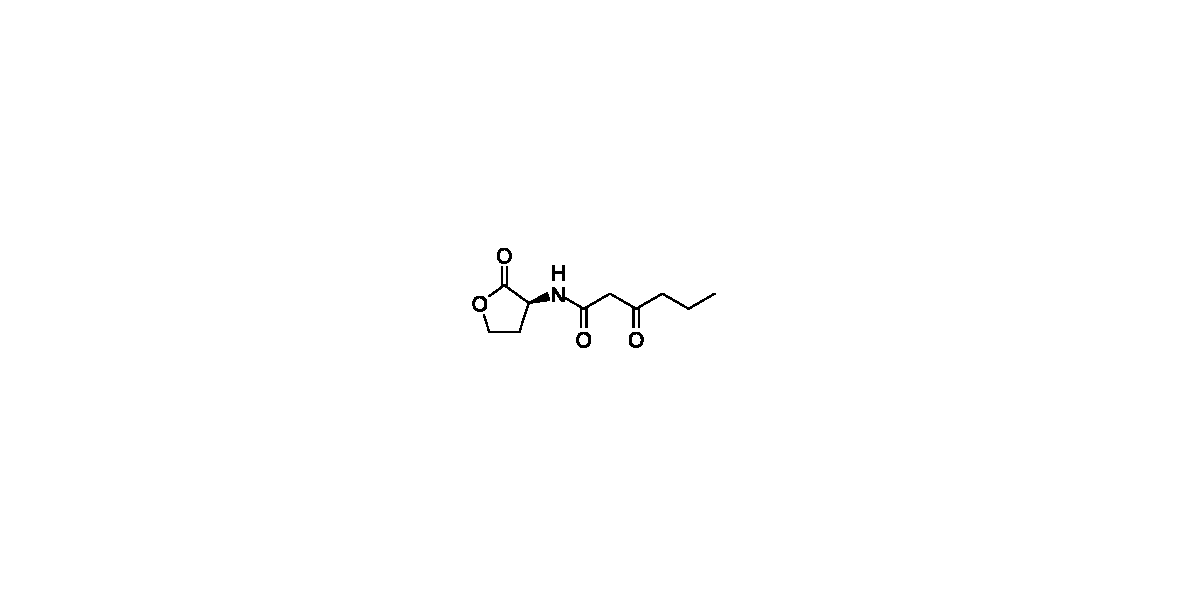
\includegraphics[scale=1]{HLO6.eps}
		\caption{3-oxo-C$_6$-HSL \compound{cmpd:HLO6}. \label{fig:HLO6}}
	\end{center}
\end{figure}

\begin{figure}[H]
	\begin{center}
		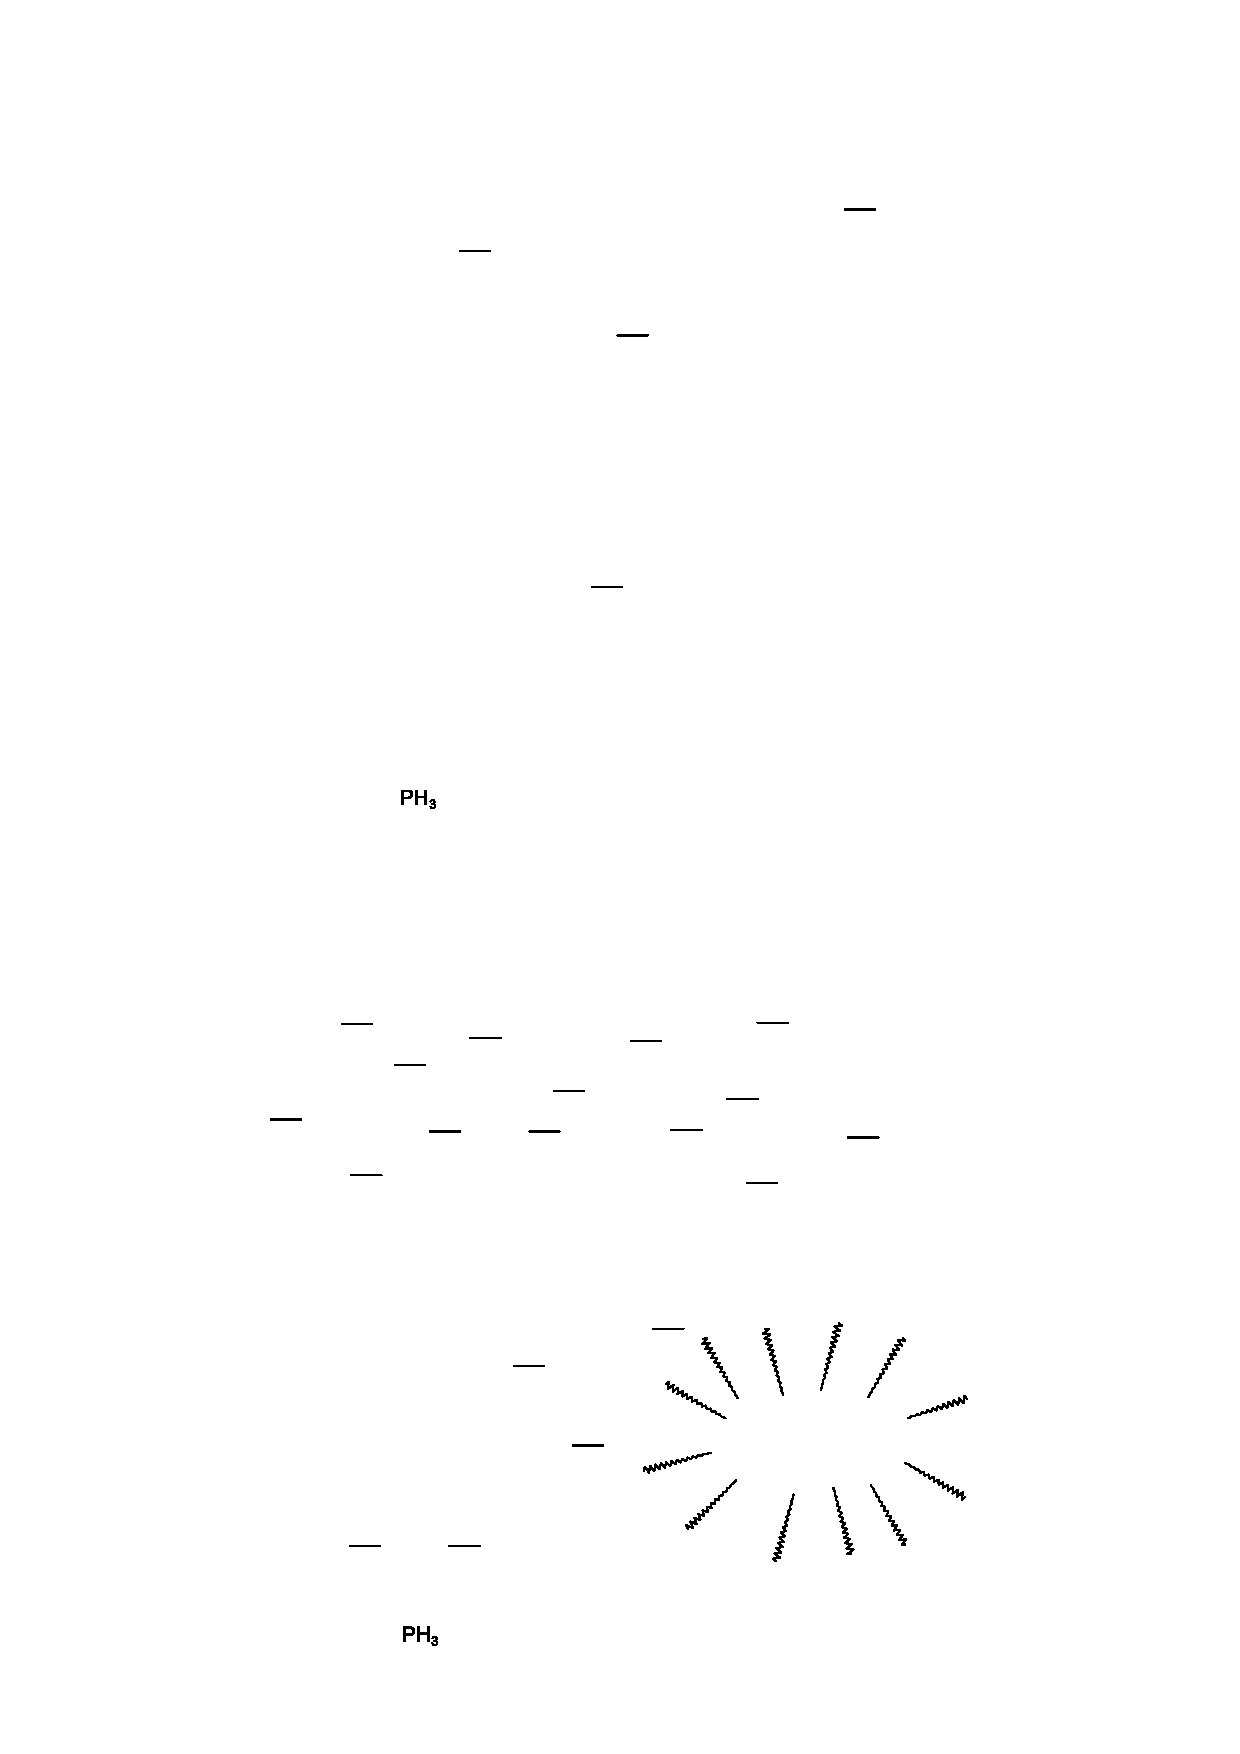
\includegraphics[scale=1]{VFQS.jpg}
		\caption{The LuxR-LuxI quorum sensing system in \textit{V. fischeri}. \label{fig:VF_QS}}
	\end{center}
\end{figure}

\subsubsubsection{Other quorum sensing systems}

Since the discovery in 1970 of the LuxR-LuxI quorum sensing system in \textit{V. fischeri}, several other mechanisms have also been discovered (it should be noted that several of the proteins mentioned in this section were first characterised in \textit{Vibrio harveyi}, and functions may be assigned by analogy to a closely-related \textit{V. harveyi} protein\cite{Miyashiro2012}). Systems using two other quorum sensing molecules, \textit{N}-octanoyl-homoserine lactone (C$_8$-HSL \compound{cmpd:HL8}) and a furanosyl borate diester (AI-2 \compound{cmpd:AI2}) have been discovered, both of which act via the \textit{luxCDABEG} system and increase luminescence by increasing luciferase production\cite{Miyashiro2012,Verma2013} (see \ref{fig:VFQS_full} and \ref{fig:VF_autoinducers}).
Additional controls in the \textit{lux} promoter region have also been discovered, which respond to O$_2$ and cAMP\cite{Miyashiro2012} (see \ref{sec:O2} and \ref{sec:cAMP}). 

The AinS–AinR system uses C$_8$-HSL \compound{cmpd:HL8}, synthesised by AinS, as its signalling molecule\cite{Lupp2003, Miyashiro2012,Gilson1995}. C$_8$-HSL \compound{cmpd:HL8} has two main effects on the quorum sensing network. Firstly, it can bind to LuxR\cite{Schaefer1996}, albeit with lower affinity than 3-oxo-C$_6$-HSL \compound{cmpd:HLO6}, leading to partial upregulation of lux operon transcription.
Secondly, it binds to the histidine kinase AinR, inhibiting its ability to phosphorylate the histidine phosphotransferase LuxU, which links into the LuxR pathway by a less direct route (see later in this section)\cite{Timmen2006}.  

%possible repression of ainSR by LuxR\cite{Kimbrough2013} (speculative, check for updates).

The LuxS–LuxP/Q system uses AI-2 \compound{cmpd:AI2}, synthesised by LuxS, as its signalling molecule\cite{Miyashiro2012,Neiditch2005,Neiditch2006} (this pathway is common to all \textit{Vibrio} species\cite{Miyashiro2012}). The receptor of AI-2 \compound{cmpd:AI2} is a complex of a two proteins, LuxP and LuxQ. LuxP is a periplasmic protein which binds AI-2 \compound{cmpd:AI2}, LuxQ is an inner membrane histidine kinase of the two-component sensor kinase family\cite{Bassler1994}. It is likely that LuxQ is constitutively dimeric, although this has not yet been demonstrated \cite{Stock2000}. 

When AI-2 \compound{cmpd:AI2} is not bound to LuxP, LuxQ autophosphorylates a histidine residue\cite{Neiditch2006}. This phosphoryl group is then transferred to an aspartic acid residue in LuxQ, and then to a histidine residue in LuxU. 

When AI-2 \compound{cmpd:AI2} binds to LuxP, this causes a major conformational change in the LuxP/Q complex, replacing one set of contacts between the proteins with another\cite{Neiditch2005,Neiditch2006} and causing the formation of an asymmetric complex of two LuxP/Q dimers. Formation of the asymmetric dimers switches the activity of LuxQ from kinase to phosphatase, which can then dephosphorylate LuxU.

At high cell density, and hence autoinducer concentration, both the AinS–AinR system and the LuxS–LuxP/Q system bring about a decrease in the amount of phosphorylated LuxU. LuxU is a phosphotransferase protein which transfers its phosphate group to an aspartic acid residue in LuxO\cite{Freeman1999}. Phosphorylated LuxO inhibits quorum sensing responses by via LuxR. Hence, at high cell densities there is a decreased amount of phosphorylated LuxU present, leading to a lack of phosphorylated LuxO, and hence increased quorum sensing responses, e.g. light production. This 'many-to-one' signalling pathway is common in bacterial two-component signalling systems \cite{Laub2007} and is found in several other \textit{Vibrionaceae}\cite{Milton2006}.

LuxO phosphate inhibits quorum sensing responses via $\sigma_{54}$-dependent transcriptional activation of \textit{qrr1}\cite{Miyamoto2000,Miyashiro2010} (despite the proximity of the \textit{luxOU} and \textit{qrr} promoters, LuxO only affects the activates the production of Qrr1 and not itself\cite{Lilley2000}). Qrr1 is a small RNA molecule (a quorum regulatory RNA or Qrr) which, with the help of Hfq, can bind to LitR RNA, leading to its degradation\cite{Miyashiro2010}. Qrr1 is the only Qrr to regulate LitR expression in \textit{V. fischeri}, and is conserved across all \textit{Vibrionaceae}\cite{Miyashiro2010}. In contrast, in other \textit{Vibrionaceae} a family of Qrrs is often used\cite{Lenz2004}.

Qrr1/Hfq-mediated degradation of LitR mRNA inhibits the production of LitR, an activator of the \textit{lux} operon. LitR binds to a region of the \textit{luxR} promoter, causing increased LuxR production and hence increased bioluminescence\cite{Fidopiastis2002}.


\begin{figure}[H]
	\begin{center}
		
\includegraphics[scale=1]{VFQS_full.jpg}
		\caption{Quorum sensing in \textit{V. fischeri}. \label{fig:VFQS_full}}
	\end{center}
\end{figure}

\begin{figure}[H]
	\begin{center}
		\schemeref[HLO6]{cmpd:HLO6}
		\schemeref[HL8]{cmpd:HL8}
		\schemeref[AI2]{cmpd:AI2}
		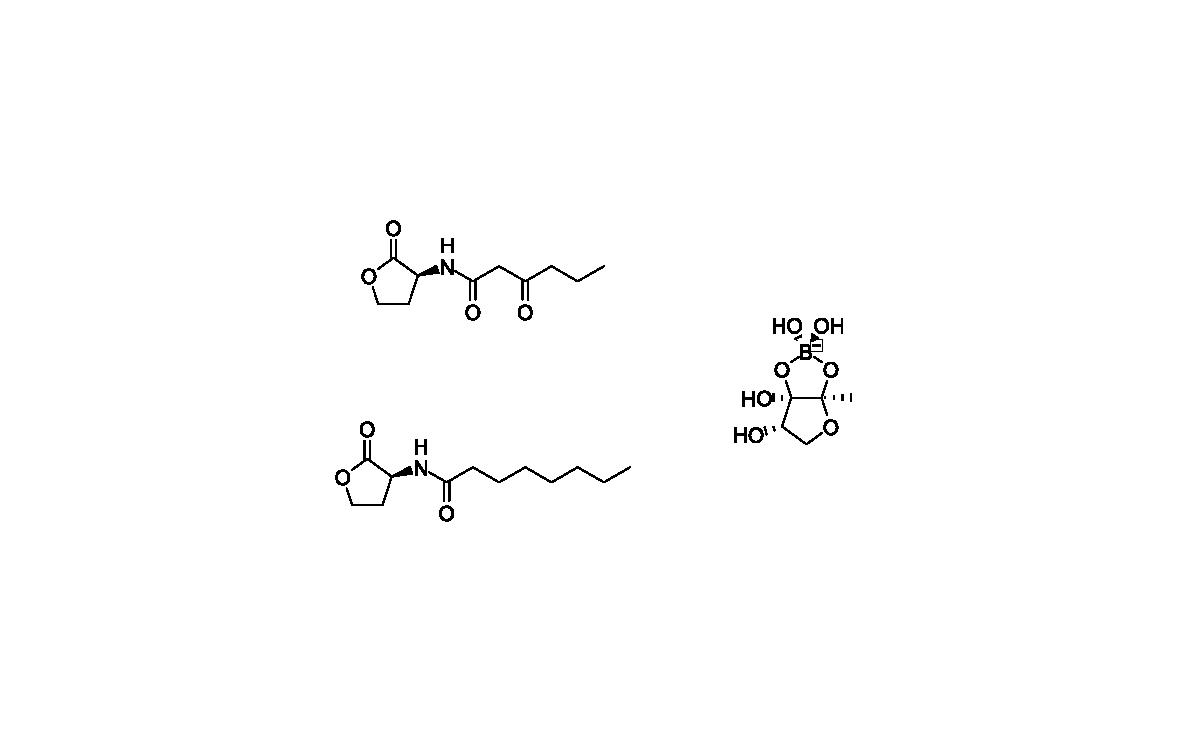
\includegraphics[scale=1]{VF_QSMs.eps}
		\caption{Quorum sensing molecules in \textit{V. fischeri}. \label{fig:VF_autoinducers}}
	\end{center}
\end{figure}

\subsubsubsection{The effect of O$_2$} \label{sec:O2}

\textit{V. fischeri} uses the ArcA-ArcB system to sense how oxygen-rich its environment is, by monitoring the redox state of various quinones produced by the cell. 
In an oxygen-rich environment, luminescence is stimulated. It is though that luminescence is used by \textit{V. fischeri} make its environment less oxidising, as luminescence consumes oxygen. 

ROS are bad and it doesn't want them\cite{Visick2000}

 ArcB is a histidine kinase which senses the redox state of the quinones. When the environment is low in oxygen or reactive oxygen species, the quinones are reduced and can stimulate ArcB to phosphorylate ArcA. ArcA is a response regulator which represses the transcription of \textit{luxICDABEG} (and to a lesser extent, \textit{luxR}). 

\subsubsubsection{The effect of cAMP} \label{sec:cAMP}

cAMP

\subsubsubsection{The purpose of multiple signalling pathways} %better title

It might reasonably be asked: why does \textit{V. fischeri} use three quorum sensing pathways rather than just one? The answer to this question lies in the bacterium's relationship with its squid host. It has been shown that the LuxS-LuxP/Q and AinS-AinR systems are important in the medium cell densities found during early colonisation of the host, whereas the LuxR-LuxI system is important at the higher cell densities found in late colonisation\cite{Lupp2003,Lupp2005}.

It has been shown that the LuxS-LuxP/Q system does not have an especially large effect on colonisation of the host squid, although it does have some effect on luminescence\cite{Lupp2004}. It has therefore been speculated that the LuxS-LuxP/Q system is more important in the colonisation of other marine invertibrates, either in their light organs\cite{Ruby1976,Reichelt1977} or as part of multi-species colonies in their guts \cite{Lupp2004,Ramesh1986}.

The AinS-AinR system has a larger effect on colonisation and luminescence, in that \textit{ainS} mutants show only 10-20 \% of wild-type luciferase activity at medium cell densities in culture (10$_8$ to 10$_8$ cells ml$_{-1}$)\cite{Lupp2003}. At the higher cell densities in the squid host (>10$_{10}$ cells ml$_{-1}$), \textit{ainS} mutants show 10-40 \% of wild-type luciferase activity, an effect which can be partially attributed to failure of the mutants to colonise the host (bacterial cell numbers are down to 20-80 \% compared to the wild type).
This failure of \textit{ainS} mutants to colonise the host is due to \textit{ain} regulation of pathways involved in early colonisation. The AinS-AinR system controls around 30 genes via LuxO and LitR\cite{Lupp2005}. \textit{ain} quorum sensing is thought to repress several motility genes, causing loss of flagella, which are initially required for normal colonisation of the host\cite{Millikan2002a,Graf1994}, but are lost as the bacteria colonise the host\cite{Ruby1993}. 
\textit{ain} quorum sensing also induces a putative exopolysaccharide, which could be important in biofilm formation inside the host, or evasion of its immune system\cite{Roberts1996}, as well as two unique.
In addition, \textit{ain} quorum sensing affects the transcription several genes involved in metabolism, and new genes of unknown function which could affect colonisation by an as yet unknown pathway.

In contrast to the AinS-AinR, the LuxI-LuxR system is only fully induced at the high cell densities found in the \textit{E. scolopes} light organ. At medium cell densities, C$_8$-HSL \compound{cmpd:HL8} is thought to be the dominant autoinducer, partially activating transcription from the \textit{lux} operon by binding to both AinR and LuxR\cite{Lupp2003}. At high cell densities, C$_8$-HSL \compound{cmpd:HL8} is displaced from LuxR by 3-oxo-C$_6$-HSL \compound{cmpd:HLO6}, leading to full light production.

\textit{lux} quorum sensing also affects the transcription of five non-\textit{lux} proteins which could potentially act as late colonisation factors\cite{Callahan2000,Qin2007}. Three of these genes, \textit{qsrP}, \textit{acfA}, and \textit{ribB}, are directly activated by LuxR/3-oxo-C$_6$-HSL\cite{Qin2007} and a strain lacking \textit{qsrP} is less effective at colonising \textit{E. scolopes} than the wild type, providing good evidence that it is a late-stage colonisation factor\cite{Callahan2000}.



ain positive feedback, LuxPQ not\cite{Lupp2004}

Which do CRP and Arc act on?
Add phos.
LitR upregulates AinS\cite{Lupp2004}





Quorum sensing has since been observed in many species of bacteria, including \textit{P. aeruginosa}, \textit{Agrobacterium tumefaciens}, \textit{Erwinia carotovora}, \textit{Streptococcus pneumoniae}, \textit{Bacillus subtilis}, \textit{S. aureus}, \textit{Vibrio harveyi}, \textit{Escherichia coli}, \textit{Myxococcus xanthus}, \textit{Salmonella enterica}, \textit{Yersinia enterocolitica}  \textit{Aeromonas} sp. and \textit{Acinetobacter} sp.\cite{Miller2001,Fuqua1994,Waters2005,Atkinson2006,Chan2011,Sauer2002,Michael2001,Ahmer2004,Nealson1970}. 
Many of these bacteria are significant causes of disease and death in humans, for example, it is estimated that in 2005 in the US \textit{S. aureus} caused 477,927 hospitalisations and 11,406 deaths\cite{Klein2007}. \textit{S. aureus} uses a peptide autoinducer know as autoinducing peptide (AIP) (see \ref{fgr:autoinducers} in \ref{sec:FutAIP}) which interacts with the \textit{agr} system leading to increased protease and toxin production\cite{Antunes2010}. \textit{P. aeruginosa} also uses quorum sensing to coordinate biofilm formation, swarming motility and virulence.






\subsubsection{\textit{Pseudomonas aeruginosa}\label{sec:PA}}

One of the most well-studied examples of QS is in \textit{P. aeruginosa}.
\textit{P. aeruginosa} is a Gram-negative opportunistic pathogen which typically infects immunocompromised individuals such as those with cystic fibrosis, neutropenia and AIDS. It can infect the pulmonary and urinary tracts as well being the most frequent cause of burn wound infections and the most frequent conloniser of medical devices such as catheters\cite{Bodey1983}.

\textit{P. aeruginosa} uses quorum sensing (QS) to coordinate biofilm formation, swarming motility and virulence. The autoinducers used by \textit{P. aeruginosa} are shown in \ref{fgr:PA_autoinducers} (HHQ \compound{cmpd:HHQ} is a precursor to PQS \compound{cmpd:PQS} but can bind to its receptor, PQSr, and hence can act as a autoinducer\cite{Xiao2006}). QS in \textit{P. aeruginosa} involves a complex interplay of the four signalling molecules and various proteins (see \ref{fgr:PA_QS})\cite{Dubern2008}. QS regulates the production of virulence factors including elastase, alkaline protease, exotoxin A, rhamnolipids, pyocyanin, lectins and superoxide dismutases, as well as regulating biofilm formation.

\textit{P. aeruginosa} has a low susceptibility to many antibiotics due to its chromosomally encoded multidrug efflux pumps: mexAB and mexXY\cite{Poole2004}. It is also difficult for drugs to cross into cells due to low cell wall permeability and biofilm formation. \textit{P. aeruginosa} may also acquire antibiotic resistance by mutation or horizontal gene transfer\cite{cornelis2008pseudomonas}. This high level of antibiotic resistance makes \textit{P. aeruginosa} an important target for drug discovery.

\begin{figure}[H]
	\begin{center}
		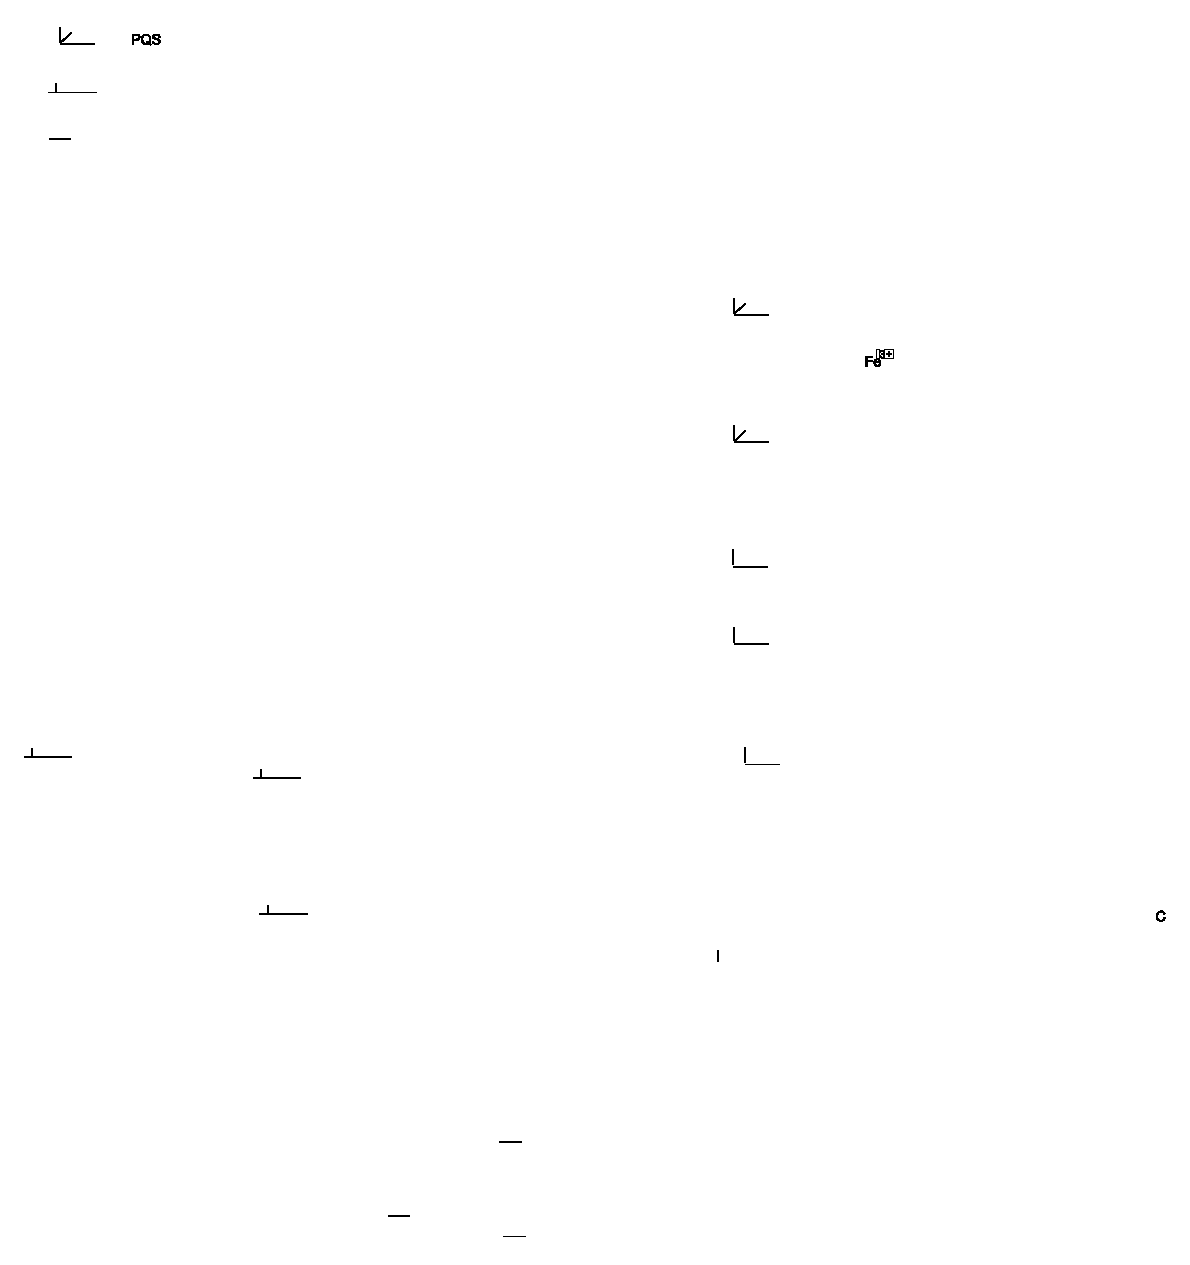
\includegraphics[width=\textwidth]{PAQS_full}
		\caption{Quorum sensing in \textit{P. aeruginosa}\cite{Dubern2008}. \label{fgr:PA_QS}}
	\end{center}
\end{figure}

%ideally save as tiff then convert to png
\todo{add biofilm to diagram, late and early development Sauer2002}

\begin{figure}[H]
	\begin{center}
		\schemeref[HL4]{cmpd:HL4}
		\schemeref[HLO12]{cmpd:HLO12}
		\schemeref[PQS1]{cmpd:PQS}
		\schemeref[HHQ1]{cmpd:HHQ}
		\schemeref[AI2]{cmpd:AI2}
		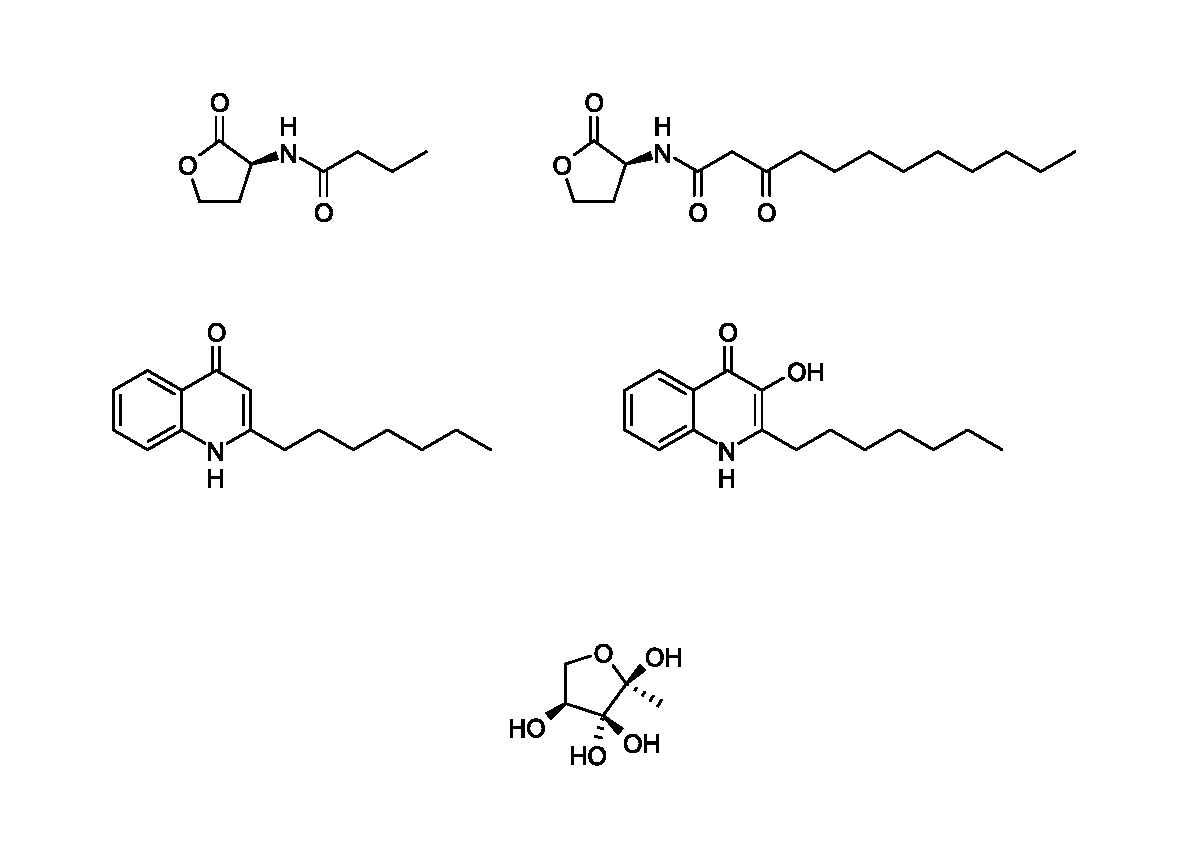
\includegraphics[scale=1]{PA_QSMs}
		\caption{\textit{P. aeruginosa} quorum sensing molecules. \label{fgr:PA_autoinducers}}
	\end{center}
\end{figure}




\subsection{Siderophores}

Siderophores are peptides or small molecules used by microorganisms to chelate iron for the purposes of 'iron mining'\cite{Hider2010}. Soluble iron is often scarce but it is crucial for many cellular processes including respiration and DNA synthesis. Siderophores are synthesised by the microorganisms and secreted into the extracellular environment where they bind to Fe$^{3+}$, often with exceptionally high affinities. The iron-bound siderophores are then brought back into the cell by active transport and the iron is released, either by reduction of the Fe$^{3+}$ to Fe$^{2+}$ or by enzymatic degradation of the siderophore. Siderophores have a wide range of structures (see \ref{fgr:Sids} and \ref{fgr:Sids_2}), possibly so one species can avoid its siderophores being taken up by another species\cite{Seyedsayamdost2012}.

\begin{figure}[H]
	\begin{center}
		\schemeref[ferri]{cmpd:ferri}
		\schemeref[fusar]{cmpd:fusar}
		\schemeref[defro]{cmpd:defro}
		\schemeref[rhodo]{cmpd:rhodo}
		\schemeref[yersin]{cmpd:yersin}
		\schemeref[entero]{cmpd:entero}
		\includegraphics[scale=1]{Siderophores}
		\caption{Iron-siderophore complexes:
		Deferoxamine \compound{cmpd:defro}\cite{Zheng2012} (\textit{Streptomyces pilosus} and \textit{Streptomyces coelicolor}), 
		rhodotorulic acid \compound{cmpd:rhodo}\cite{Carrano1978} (\textit{Rhodotorula pilimanae}),
		fusarinine C \compound{cmpd:fusar}\cite{Hossain1980} (\textit{Fusarium roseum}),
		enterobactin \compound{cmpd:entero}\cite{Zheng2012} (\textit{Escherichia coli} and enteric bacteria),
		ferrichrome \compound{cmpd:ferri}\cite{vanderHelm1980} (\textit{Ustilago sphaerogena}, \textit{U. maydis}, \textit{Aspergillus niger}, \textit{A. quadricintus}, \textit{A. duricaulis} and \textit{Penicillium resticolosum}),
		yersiniabactin \compound{cmpd:yersin}\cite{Zheng2012} (\textit{Yersinia pestis}).
		\label{fgr:Sids}}
	\end{center}
\end{figure}

\begin{figure}[H]
	\begin{center}
		\schemeref[pyo]{cmpd:pyo}
		\schemeref[pyoch]{cmpd:pyoch}
		\includegraphics[scale=1]{Siderophores_2}
		\caption{Iron-siderophore complexes:
		Pyochelin \compound{cmpd:pyo}\cite{Schlegel2006} (\textit{P. aeruginosa}),
		Pyoverdine \compound{cmpd:pyoch}\cite{Zheng2012} (\textit{P. aeruginosa}). Note that pyoverdine \compound{cmpd:pyoch} is a tetradentate ligand, hence the iron ion has two sites which can bind other ligands. \label{fgr:Sids_2}}
	\end{center}
\end{figure}

\subsection{Sideromycins}


Siderophore-antibiotic conjugates are produced naturally by some bacteria and are known as sideromycins\cite{Page2013} (see \ref{fgr:SidMys}). Bacteria produce these molecules to attack other bacteria by hijacking their siderophore uptake mechanisms to introduce toxic compounds. 

For example, albomycin \compound{cmpd:albo} (see \ref{fgr:SidMys}) is a sideromycin produced by \textit{Actinomyces subtropicus} and \textit{Streptomyces griseus}\cite{Hartmann1979,Fiedler1985} which has been used to treat infections caused by various bacteria including \textit{Yersinia enterocolitica} and \textit{Streptococcus pneumoniae} in mice and humans\cite{Gause1955,Pramanik2007}. 
Albomycin \compound{cmpd:albo} contains a siderophore coupled to a nuceloside antibiotic via a peptide linker. 
The siderophore section is structurally similar to ferrichrome \compound{cmpd:ferri} (see \ref{fgr:Sids}), a siderophore produced by various fungi, but also taken up by bacteria including \textit{Escherichia coli}, \textit{Salmonella typhimurium} and \textit{P. aeruginosa}\cite{vanderHelm1980,Hannauer2010}.
It has been shown that because of the structural similarity to ferrichrome \compound{cmpd:ferri}, \textit{E. coli} will also take up albomycin \compound{cmpd:albo}\cite{Hartmann1979}.
The linker is hydrolysed in the cytoplasm of the \textit{E. coli}, releasing the active nuceloside antibiotic. This leads to 500-fold concentration of the antibiotic within the \textit{E. coli} cells, enough to have significant effect on growth.

The success of albomycin\cite{Gause1955} and other sideromycins such as salmycin A\cite{Hider2015,Braun2009} and ferrimycin A1\cite{Sackmann1962,Gottlieb2012} has served as encouragement to many researchers to explore synthetic siderophore-antibiotic conjugates, which will be discussed in the next section. 

%Albomycin kills in vitro: staphylococci, Escherichia coli, Aerobacter aerogenes,Sarcina subflava, and Bacillus subtilis (Gause and Brazhnikova, 1951). Further, pneumococci, Klebsiella, dysentery bacilli, and some (but not all) strains of Streptococcus pyogenes are very sensitive. 

\begin{figure}[H]
	\begin{center}
		\schemeref[albo]{cmpd:albo}
		\schemeref[ferrim]{cmpd:ferrim}
		\schemeref[sal]{cmpd:sal}
		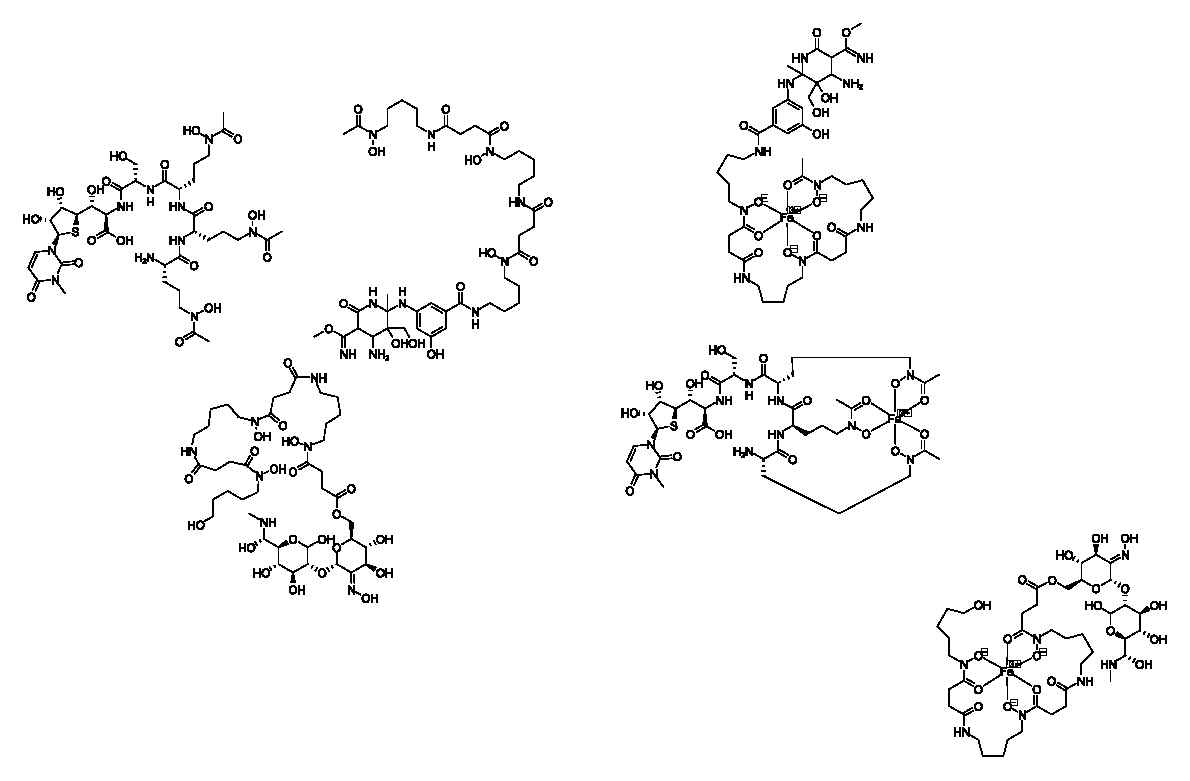
\includegraphics[scale=1]{SidMys}
		\caption{Iron-sideromycin complexes: Albomycin \compound{cmpd:albo}\cite{Benz1982,Hider2015} (\textit{Actinomyces subtropicus} and \textit{Streptomyces griseus}), salmycin A\cite{Hider2015,Braun2009} (\textit{Streptomyces violaceus}) and ferrimycin\cite{Hider2015} (\textit{Streptomyces griseoflavus}). \label{fgr:SidMys}}
	\end{center}
\end{figure}

\subsection{Synthetic siderophore-antibiotic conjugates}

Sideromycins served as inspiration for the design, synthesis and biological evaluation of a wide range of synthetic siderophore-antibiotic conjugates\cite{Page2013}. Antibiotics used include $\beta$-lactams\cite{Mollmann2009,Dini2000,Kline2000}, nucleosides\cite{Lu1999}, glycopeptides\cite{Ghosh1996} and macrolides\cite{Ghosh1995}. Sideromycin-fluoroquinolone conjugates have also been studied by several groups\cite{Md-Saleh2009,Rivault2007,Ji2012}, including conjugates with linkers which can be cleaved\cite{Rivault2007,Ji2012} in a similar manner to albomycin\cite{Hartmann1979}. Some of these showed comparable activity to the parent antibiotic, but it is not clear whether attachment of the siderophore improved uptake or whether the conjugates acted as classical prodrugs.

$\beta$-lactam-sideromycin conjugates have been more widely investigated and show good activity \textit{in vitro}, however, resistance can evolve by loss of the TonB transporter or of the relevant siderophore receptor, e.g. Cir and Fiu for catecholate siderophores or FhuA for hydroxamate siderophores\cite{Page2013}. 
Recently a conjugate (Ent-Amp \compound{cmpd:Ent-Amp}, see \ref{fgr:SidABs}) of enterobactin and ampicillin joined using a copper(I)-catalyzed azide-alkyne cycloaddition has been shown to have increased activity against pathogenic \textit{E. coli} when compared to native ampicillin\cite{Zheng2014}. 
Other work has focused on monocyclic $\beta$-lactams, for example pirazmonam \compound{cmpd:Pir} and U-78608 \compound{cmpd:U-78}, which show high potency against Gram-negative bacteria including \textit{P. aeruginosa},\cite{Zurenko1990,Harrington2012}. Monocyclic $\beta$-lactams are generally fairly stable to $\beta$-lactamase activity, which is an advantage compared with many bicyclic $\beta$-lactams.

Three siderophore-antibiotic conjugates are reported as being in clinical trials\cite{Schalk2017}: MC-1 \compound{cmpd:MC-1}\cite{McPherson2012}, BAL30072 \compound{cmpd:BAL}\cite{Page2013} (see \ref{fgr:SidABs}) and cefiderocol \compound{cmpd:S-64}\cite{Ito2018,Saisho2018}\todo{pre-release paper}.

MC-1 \compound{cmpd:MC-1} is reported as being "in clinical phases of development"\cite{Schalk2017}, but no reports of studies in humans could be found. However, experiments in mice have been promising\cite{McPherson2012}.
BAL30072 \compound{cmpd:BAL} is a siderophore-$\beta$-lactam conjugate which showed initial promise as it is a poor substrate for $\beta$-lactamases, and resistance due to loss of transport proteins is infrequent\cite{Page2013}. However, it is unclear whether it will progress further in trials as it causes liver toxicity\cite{Paech2017}. 
Cefiderocol \compound{cmpd:S-64} is a cephalosporin-catechol conjugate in phase 1 trials. Recent results indicate that 'single and 35 multiple intravenous doses of cefiderocol at up to 2000 mg were well tolerated in healthy 36 subjects'\cite{Saisho2018}.

These examples show that siderophore-antibiotic conjugates are a promising strategy to deliver antibiotics across bacterial membranes, but it is worth noting that conjugation to a siderophore may lead to loss of activity, or resistance may be acquired by loss of transport proteins. Encouragingly though, albomycin \compound{cmpd:albo}-resistant mutants have been shown to be less virulent \cite{Pramanik2007}, indicating that bacteria may lose out either by susceptibility to the antibiotic or by loss of fitness due to decreased iron transport. 

Building on these positive examples, it is hoped that the strategy of conjugating a molecule which is important for virulence with an antibiotic can be extended to conjugates of autoinducers and antibiotics in a similar 'Trojan horse' approach.

\begin{figure}[H]
	\begin{center}
		\schemeref[bal]{cmpd:BAL}
		\schemeref[mc1]{cmpd:MC-1}
		\schemeref[ln]{cmpd:LN}
		\schemeref[s64]{cmpd:S-64}
		\schemeref[entamp]{cmpd:Ent-Amp}
		\schemeref[u78]{cmpd:U-78}
		\schemeref[pir]{cmpd:Pir}
		\includegraphics[scale=1]{SidABs}
		\caption{Ent-Amp \compound{cmpd:Ent-Amp}\cite{Zheng2014}, 
		pirazmonam \compound{cmpd:Pir}\cite{Zurenko1990,Harrington2012}, 
		U-78608 \compound{cmpd:U-78},\cite{Zurenko1990,Harrington2012}, 
		MC-1 \compound{cmpd:MC-1}\cite{McPherson2012},  
		BAL30072 \compound{cmpd:BAL}\cite{Page2013}
		and cefiderocol \compound{cmpd:S-64}\cite{Ito2018,Saisho2018}.
		\label{fgr:SidABs}}
	\end{center}
\end{figure}



\subsection{Autoinducer-antibiotic conjugates}

This study extends the conjugation strategy discussed above by creating autoinducer-antibiotic conjugates. It was hypothesised that attaching an autoinducer to a known antibiotic could lead to increased cellular retention of the antibiotic, and could potentially restore function in resistant strains.
The work is divided into two main sections. The first section focuses on conjugates of three \textit{P. aeruginosa} autoinducers (see \ref{fgr:3PA_AIs}) with ciprofloxacin and trimethoprim (see \ref{fgr:ABs}).
The second section focuses on conjugates of homoserine lactone analogues with ciprofloxacin (see \ref{sec:AIA_intro}).

\subsubsection{Autoinducers}

The \textit{P. aeruginosa} autoinducers (see \ref{fgr:PA_autoinducers}) were chosen as \textit{P. aeruginosa} is a significant human pathogen which shows high antibiotic resistance and utilises quorum sensing to coordinate pathogenic behaviours (see \ref{sec:PA}). 

The five known \textit{P. aeruginosa} autoinducers have different transport mechanisms in and out of cells:
The mechanism is not well known for HHQ \compound{cmpd:HHQ} or AI-2 \compound{cmpd:AI2}, 
PQS is exported in vesicles\cite{Florez2017},
C$_4$-HSL \compound{cmpd:HL4} passively diffuses in and out of cells\cite{Pearson1999}, and
3-oxo-C$_12$-HSL \compound{cmpd:HLO12} is taken up passively, accumulates in the cell membrane and is actively pumped out by efflux pumps.

The difference in transport mechanism for C$_4$-HSL \compound{cmpd:HL4} and 3-oxo-C$_12$-HSL \compound{cmpd:HLO12} is thought to be largely due to chain length rather than the 3-oxo modification, as a shorter-chain version, 3-oxo-C$_6$-HSL \compound{cmpd:HLO6} has been shown to be freely diffusable through V. fischeri membranes\cite{Kaplan1985}.

%The transport of 3-oxo-C$_12$-HSL \compound{cmpd:HLO12} is noteworthy, as it is exported by efflux pumps which are also involved in the export of antibiotics, including ciprofloxacin.

Upregulation of the MexAB-OprM efflux system leads to increased efflux of 3-oxo-C$_12$-HSL \compound{cmpd:HLO12}\cite{Evans1998}.
The removal of 3-oxo-C$_12$-HSL \compound{cmpd:HLO12} from the cell leads to decreased production of additional 3-oxo-C$_12$-HSL \compound{cmpd:HLO12} (as the positive feedback loop is disrupted, see \ref{sec:PA}), and hence decreased production of pyocyanin, elastase and casein protease. 
It is expected that MexAB-OprM upregulation would also disrupt biofilm formation as a decrease in 3-oxo-C$_12$-HSL \compound{cmpd:HLO12} levels would disrupt both Las- and Rhl-mediated quorum sensing\cite{blah}, but no direct studies of this could be found.

HHQ \compound{cmpd:HHQ}, PQS \compound{cmpd:PQS} and C$_4$-HSL \compound{cmpd:HL4} (see \ref{fgr:PA_autoinducers}) derivatives were chosen as they were deemed most synthetically tractable.


\subsubsection{Antibiotics}

Ciprofloxacin \compound{cmpd:Cip} and trimethoprim \compound{cmpd:Tri} (see \ref{fgr:ABs}) were chosen as the antibiotic sides of the conjugates.
 
Ciprofloxacin \compound{cmpd:Cip} is second-generation fluoroquinolone antibiotic used to treat both Gram-positive and Gram-negative bacterial infections including \textit{P. aeruginosa}\cite{Oliphant2002,Macgowan1999}.
\textit{P. aeruginosa} biofilms are more resistant to ciprofloxacin \compound{cmpd:Cip} than planktonic cells\cite{Evans1991}.

%, and this difference is more pronounced at high growth rates\cite{Evans1991}.
%In addition, the resistance of intact biofilms is significantly higher than that of resuspended biofilm cells, suggesting that organization of the cells within the biofilm confers resistance\cite{Evans1991}. 
%However, there are conflicting reports on whether \textit{P. aeruginosa} biofilms impede the diffusion of ciprofloxacin\cite{Suci1994,Shigeta1997,Kumon1994}, and regardless it has been shown that limited antibiotic diffusion through the biofilm is not the primary mechanism of resistance of \textit{P. aeruginosa} biofilms against ciprofloxacin \compound{cmpd:Cip}\cite{Walters2003}.
%Instead it is likely that poor oxygen penetration and low metabolic activity within the interior of the biofilm is responsible for the low antibiotic activity.
%This is expected for ciprofloxacin \compound{cmpd:Cip}, as it works by inhibiting DNA gyrase and topoisomerase IV, thereby inhibiting cell division.

Ciprofloxacin \compound{cmpd:Cip} enters \textit{P. aeruginosa} by diffusion\cite{Celesk1989}, but is pumped out by efflux pumps\cite{Poole2000}. In the planktonic state several efflux pumps are known to pump out ciprofloxacin \compound{cmpd:Cip}, including MexAB–OprM, MexCD–OprJ, MexEF–OprN, MexXY–OprM, MexJK–OprM and MexVW–OprM\cite{Poole2004}. 
However, in biofilms only MexEF-OprN has an effect\cite{DeKievit2001}.



It is hoped that \textit{P. aeruginosa} would develop resistance to a conjugate of HSL and ciprofloxacin \compound{cmpd:Cip} by upregulation of the MexAB-OprM pump. This would also lead to increased export of 3-oxo-C$_12$-HSL \compound{cmpd:HLO12}, thus disrupting the quorum-sensing system and hence biofilm formation and virulence.

It is hoped that the HSL group would make the conjugate a poor substrate of MexEF–OprN (the sole exporter of ciprofloxacin \compound{cmpd:Cip} in biofilms\cite{DeKievit2001} and not an exporter of HSLs\cite{blah}) as this would lead to accumulation of the conjugate within cells and hence cell death.

%Is 3-oxo-C$_12$-HSL \compound{cmpd:HLO12} a substrate of other pumps? Maybe HI \cite{Poole2004}

%synonyms PAI-1 = 3-oxo =oddhl
%Iron important for virulence
%change c4 anagolges to HSL analogues
%chain length active transport
%cleavable sid conjugates

%\textit{P. aeruginosa} acquires resistance to ciprofloxacin \compound{cmpd:Cip} by two main routes: mutation in gyrase or topoisomerase IV, and mutations in efflux pumps\cite{Jalal2000}. 

%It is often assumed that biofilms have higher resistance to antibiotics than planktonic cells, however this may not necessarily be the case for \textit{P. aeruginosa}\cite{Spoering2001}.

Trimethoprim (see \ref{fgr:ABs}) is a dihydrofolate reductase inhibitor used primarily to treat bladder infections\cite{Brogden1982}. It is active against several significant human pathogens including \textit{Streptococcus pneumoniae} and \textit{Haemophilus influenzae}. It was primarily chosen in this study as it was easy to functionalise.

These results demonstrate that the mexABoprM multidrug efflux system is mainly responsible for the intrinsic resistance of P. aeruginosa to TMP\cite{Kohler1996}

%\todo{It doesn't kill Staph A...} 

\begin{figure}[H]
	\begin{center}
		\schemeref[Cip]{cmpd:Cip}
		\schemeref[Tri]{cmpd:Tri}
		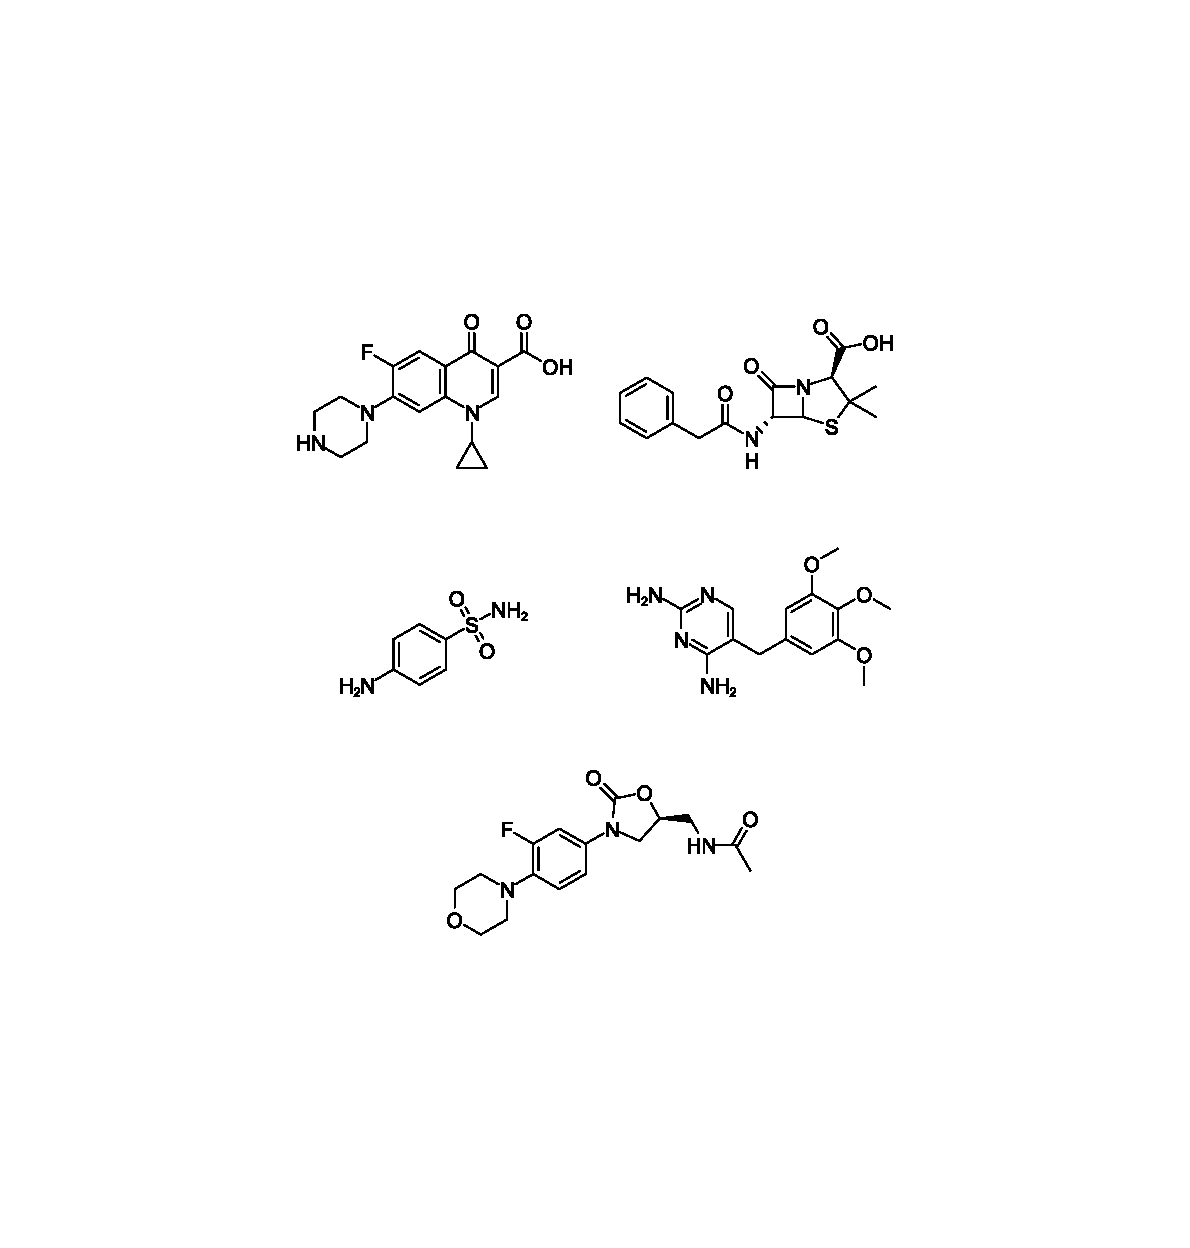
\includegraphics[scale=1]{ABs}
		\caption{The antibiotics used in this section. \label{fgr:ABs}}
	\end{center}
\end{figure}

\todo{consistency on figure captions/labelling of molecules}

\subsubsection{Synthesis of the conjugates}

A copper(I)-catalysed azide-alkyne cycloaddition\cite{Tornoe2002,ANIE:ANIE2596}, commonly referred to as a click reaction (although this is a more general term), was used to join each combination of autoinducer and antibiotic together (see \ref{sch:QSAB_synth_overv}). This modular approach would allow the library to be easily expanded by adding more autoinducers or antibiotics, or indeed other groups such as siderophores, fluorescent or affinity tags, or resin beads. 

\begin{scheme}[H]
	\begin{center}
		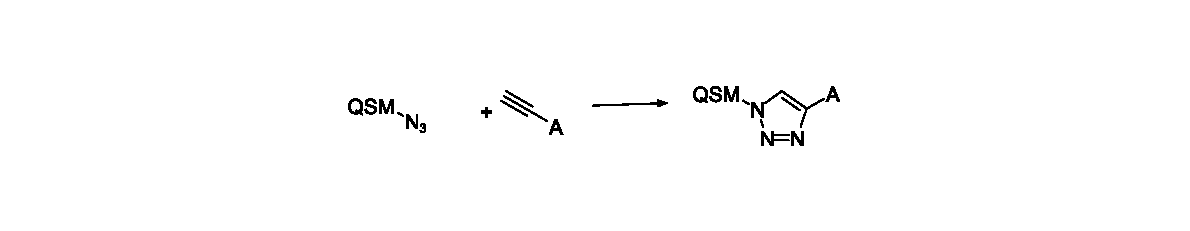
\includegraphics[scale=1]{QSAB_synth_overv}
		\caption{The construction of the triazole-linked autoinducer-antibiotic conjugate library using a copper(I)-catalysed azide-alkyne cycloaddition. \label{sch:QSAB_synth_overv}}
	\end{center}
\end{scheme}




\subsection{Autoinducer analogue-ciprofloxacin conjugates\label{sec:AIA_intro}}

Following on from the library of compounds based on \textit{P. aeruginosa} autoinducers, a series of conjugates based on \textit{analogues} of C$_4$-HSL were planned. This strategy was inspired by a paper\cite{Ganguly2011} and patent\cite{Iyer2012} by Ganguly \textit{et al.}, who synthesised and characterised a conjugate \compound{cmpd:SHL4CipMe} of methyl ciprofloxacin with homocysteine thiolactone (see \ref{fig:SHL4CipMe}). Homocysteine thiolactone is an analogue of homoserine lactone with the ring oxygen replaced by sulfur, and has been used as the head group in several other known quorum sensing modulators\cite{Eberhard1986,Schaefer1996,Passador1996,Smith2003,Chhabra1993,McInnis2011,Geske2007,Janssens2007}.\todo{show compounds it's in and describe?}
\todo{(good it has Me so it accumulates in membranes like 3 oxo?)}

\begin{figure}[H]
	\begin{center}
		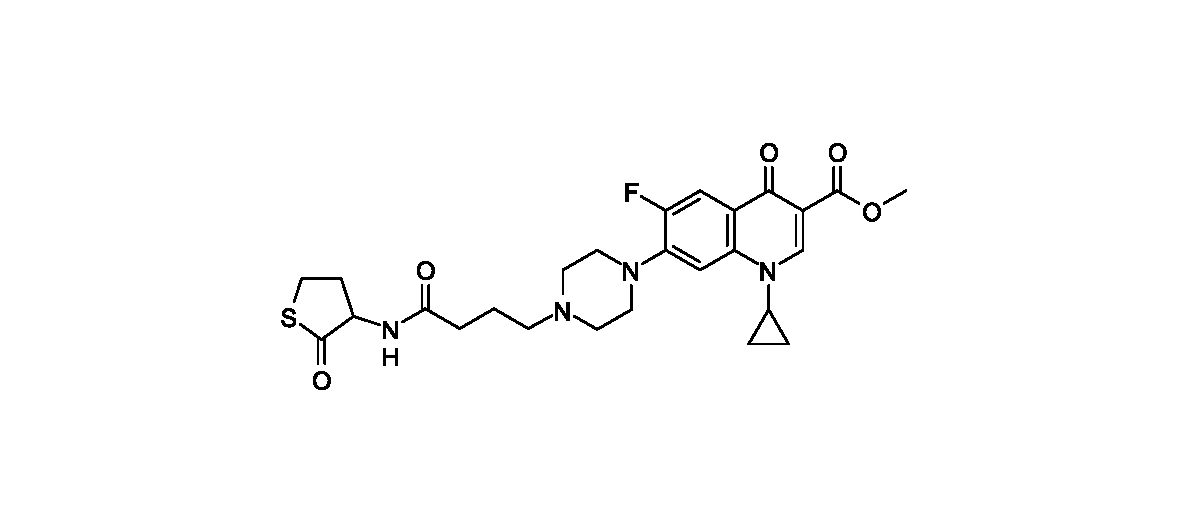
\includegraphics[scale=1]{SHL4CipMe}
		\caption{The HCTL-CipMe conjugate \compound{cmpd:SHL4CipMe} studied by Ganguly \textit{et al.}\cite{Ganguly2011,Iyer2012}.\label{fig:SHL4CipMe}}
	\end{center}
\end{figure}


As part of their characterisation of the HCTL-CipMe conjugate \compound{cmpd:SHL4CipMe}, Ganguly \textit{et al.} found the minimum inhibitory concentration (MIC) of the conjugate in \textit{P. aeruginosa} under standard planktonic conditions. 
The MIC was found to be ten times higher for the conjugate vs. ciprofloxacin (50 vs. 5 $\mu$m), indicating that the conjgate was less effective than ciprofloxacin under planktonic conditions. 

Ganguly \textit{et al.} then investigated the effect of the conjugate on biofilms. 
The conjugate and ciprofloxacin were first added to dilute \textit{P. aeruginosa} liquid culture at 25 $\mu$m. 
As expected, the culture failed to grow and form biofilm in the presence of ciprofloxacin, but did grow in the presence of the conjugate \compound{cmpd:SHL4CipMe}. 
They then incubated cultures for 24 h, to allow biofilms to grow, before adding the compounds. In contrast, they found that the conjugate \compound{cmpd:SHL4CipMe} disrupted the biofilm more effectively than ciprofloxacin. 
When the biofilm was grown for 48 or 72 hours the conjugate had similarly disruptive effects, whereas ciprofloxacin `did not show any significant antibacterial activity'.

These results are exciting as they hint that an autoinducer conjugate might be able to combat an established \textit{P. aeruginosa} infection more effectively than the unmodified antibiotic. 
Ganguly \textit{et al.} suggest that their conjugate is more effective than ciprofloxacin in penetrating biofilms, and/or better at avoiding being pumped out by multidrug efflux pumps. They posit that this could be due to the thiolactone head, as they also showed that unconjugated C$_4$-HCTL \compound{cmpd:SHL4} (see \ref{fig:HL_SHL}) has `either enhanced uptake or functional activity' when compared with C$_4$-HSL \compound{cmpd:HL4}. 

\begin{figure}[H]
	\begin{center}
		\schemeref[HL4]{cmpd:HL4}
		\schemeref[SHL4]{cmpd:SHL4}
		\includegraphics[scale=1]{HL_SHL}
		\caption{
		C$_4$-HSL \compound{cmpd:HL4} and C$_4$-HCTL \compound{cmpd:SHL4}. Note that Ganguly \textit{et al.} tested the \textit{S} enantiomer of C$_4$-HCTL \compound{cmpd:SHL4}, but used a racemic mixture in their HCTL-CipMe conjugate.
		\label{fig:HL_SHL}}
	\end{center}
\end{figure}

\todo{is it racemic?}

While the results found by Ganguly \textit{et al.} show promise, they only test one conjugate, and do not include controls to show that the HCTL group specifically is necessary for the enhanced effect.
It was therefore decided to build on this work by synthesising a series of ciprofloxacin conjugates with head groups known as part of quorum sensing modulators\cite{Galloway2011,Hodgkinson2012a}.\todo{read these again, put ones I didn't do in further work}

The activity of the chosen head groups against \textit{P. aeruginosa} receptors when coupled with the native C$_4$ and 3-oxo-C$_12$ tails is summarised in \ref{tbl:head_groups}. It is hoped that high activity of these molecules should correlate with high activity of their ciprofloxacin conjugates.
This is not a comprehensive list of active head groups, and other possible choices are covered in \ref{sec:future}.

\begin{table}[H]
  \centering
\begin{tabular}{|P{0.18\textwidth}|p{0.32\textwidth}|p{0.32\textwidth}|}
\hline 
 \vspace{8px}\textbf{Head group} & \vspace{0px}\centering\includegraphics[scale=1]{C4_tail} & \centering\arraybackslash\vspace{0px}\includegraphics[scale=1]{oddhl_tail} \\ 
\hline 
 \vspace{0px}\includegraphics[scale=1]{SHL_head} & Partial agonist and antagonist against LasR\cite{McInnis2011}. Shown to increase biofilm formation in \textit{P. aeruginosa}\cite{Ganguly2011}.
 & Strong agonist against LasR, with comparable activity to the native ligand\cite{Smith2003,Boursier2018,Passador1996,McInnis2011}. \\ 
 %L vs racemate doesn't matter \cite{McInnis2011} D might actually do better?
 %check receptor. hydrolytic stability is higher for SHL. is it racemic in Ganguly?
 %Some evidence that \textit{R} enantiomer is more potent\cite{McInnis2011}.
%\hline 
% \vspace{0px}\includegraphics[scale=1]{2MeOA_head} 
% & Not yet studied. 
% & Not yet studied. \\  
\hline 
 \vspace{0px}\includegraphics[scale=1]{3MeOA_head} 
 & Partial agonist against LasR\cite{Hodgkinson2012a}. 
 & Strong antagonist against LasR\cite{Hodgkinson2012a}. \\ 
\hline 
 \vspace{0px}\includegraphics[scale=1]{HOcy5_S_head} 
 & Poor agonist and antagonist against RhlR\cite{Smith2003a,Jog2006}.
 & Strong antagonist against LasR\cite{Smith2003a}.\\ 
\hline 
 \vspace{0px}\includegraphics[scale=1]{Ocy5_S_head} 
 & Strong agonist against RhlR\cite{Smith2003a}. \textit{SS} enantiomer is more potent\cite{Jog2006}.
 & Partial agonist against LasR\cite{Smith2003a}. \\ 
\hline 
 \vspace{0px}\includegraphics[scale=1]{HOcy6_S_head} 
 & Strong agonist against RhlR\cite{Smith2003a}. \textit{SS} enantiomer is more potent, with comparable activity to the native ligand\cite{Jog2006}.
 & Strong agonist against LasR\cite{Smith2003,Smith2003a}. \textit{SS} enantiomer is more potent, with comparable activity to the native ligand\cite{Jog2006}.\\ 
\hline 
 \vspace{0px}\includegraphics[scale=1]{Ocy6_S_head} 
 & Strong agonist against RhlR\cite{Smith2003a}. \textit{SS} enantiomer is more potent\cite{Jog2006}.
 & Partial antagonist against LasR\cite{Smith2003a}. Shown to reduce biofilm formation in \textit{P. aeruginosa}\cite{Smith2003a}.\\ 
\hline 
\end{tabular}
\caption{Activities of autoinducers containing the chosen head groups when coupled with C$_4$ or 3-oxo-C$_12$ tails.\label{tbl:head_groups}} 
\end{table}

%The formation of biofilms can drastically increase MIC for many antibiotics \cite{Ceri1999}. For ciprofloxacin in \textit{P. aeruginosa} the MIC increases by 16 fold according to Ceri \textit{et al.} 

%Ganguly \textit{et al.} used Bac-Light Live/Dead staining and confocal microscopy to image the biofilms, whereas so far I have used crystal violet staining. Crystal violet does not differentiate between live or dead cells, and so might not pick up on the antibacterial effects of compounds. However, their confocal microscopy results show a quantifiable decrease in biofilm thickness, and it may be possible to detect this using crystal violet.

%
%\newpage
%
%\section{Aims}
%
%The aim of this project is to produce a library of autoinducer-antibiotic conjugates with the hope of increasing the potency of the drugs and possibly restoring their antibacterial action against resistant strains. The library is built from a collection of \textit{P. aeruginosa} autoinducer analogues with azide groups attached and a collection of antibiotics with alkyne groups attached. These collections will then be combined using a copper(I)-catalysed azide-alkyne cycloaddition\cite{Tornoe2002,ANIE:ANIE2596} reaction to form the library of final conjugates. This approach has recently been used by Zheng \textit{et al.}\cite{Zheng2014} to join the siderophore enterobactin \compound{cmpd:entero} (see \ref{fgr:Sids}) with ampicillin or amoxicillin (see \ref{fgr:pen_anas} in \ref{sec:Futpen}).
%
%\subsection{Quorum sensing molecule-antibiotic conjugates}
%
%A copper(I)-catalysed azide-alkyne cycloaddition\cite{Tornoe2002,ANIE:ANIE2596}, commonly referred to as a click reaction although this is a more general term, will be used to join each combination of autoinducer and antibiotic together (see \ref{sch:QSAB_synth_overv}). This modular approach allows the library to be easily expanded by adding more QMSs or antibiotics, or indeed other groups such as siderophores, fluorescent or affinity tags, or resin beads. The library will then be screened for antibiotic activity against \textit{P. aeruginosa} and other pathogenic bacteria.
%
%\begin{scheme}[H]
%	\begin{center}
%		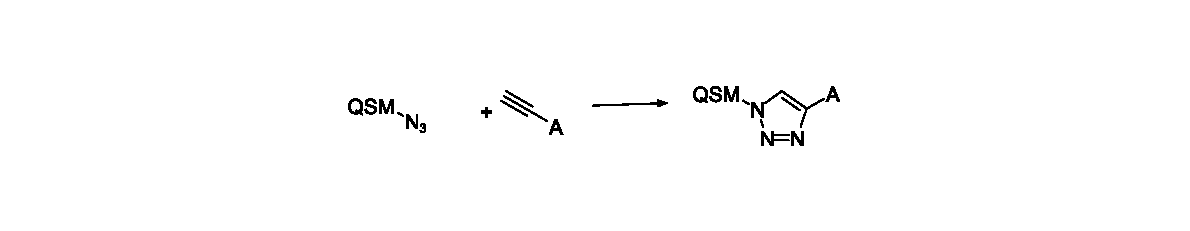
\includegraphics[scale=1]{QSAB_synth_overv}
%		\caption{The proposed construction of the library using a copper(I)-catalysed azide-alkyne cycloaddition. \label{sch:QSAB_synth_overv}}
%	\end{center}
%\end{scheme}
%
%\subsection{Quorum sensing molecule analogues}
%
%The four main autoinducers used by \textit{P. auruginosa} are shown in \ref{fgr:PA_autoinducers} in \ref{sec:PAautoinducers}. 
%We have decided to focus initially on the synthesis of azido analogues of C$_4$-HSL \compound{cmpd:HL4}, HHQ \compound{cmpd:HHQ} and PQS \compound{cmpd:PQS}. A synthesis of an azido analogue of 3-oxo-C$_12$-HSL \compound{cmpd:HLO12} has also been planned (see \ref{sch:HLO12N3_synth} in \ref{sec:Fut_HLO12}) and will be attempted in due course.
%
%The structure-activity relationships in PQS have been previously studied \cite{Hodgkinson2010}, and 5 and 6 positions could be substituted without significantly affecting the activity of the PQS molecule (see \ref{fgr:PQS_num}). Placing of the azide group at position 6 was chosen for synthetic reasons and the azide group was placed in the equivalent position in the HHQ analogue (see \ref{fgr:HHQPQSaz}).
%
%Alteration of the lactone group of C$_4$-HSL and other HSL derivatives is known to significantly decrease activity, especially where the number of H-bond donors or acceptors is altered \cite{Galloway2011}. Hence, the azide group will be included on the tail of C$_4$-HSL. Acyl tail length is known to play an important role in affinity, so we have decided to synthesise three analogues of C$_4$-HSL: azido-C$_2$-HSL \compound{cmpd:HL2N3}, azido-C$_4$-HSL \compound{cmpd:HL4N3} and azido-C$_6$-HSL \compound{cmpd:HL6N3} (see \ref{fig:HL_anas}).
%
%
%
%\begin{figure}[H]
%	\begin{center}
%		\schemeref[PQS]{cmpd:PQS}
%		\includegraphics[scale=1]{PQS_num}
%		\caption{The atom numbering in PQS \compound{cmpd:PQS}. \label{fgr:PQS_num}}
%	\end{center}
%\end{figure}
%
%\begin{figure}[H]
%	\begin{center}
%		\schemeref[azHHQ]{cmpd:azHHQ}
%		\schemeref[azPQS]{cmpd:azPQS}
%		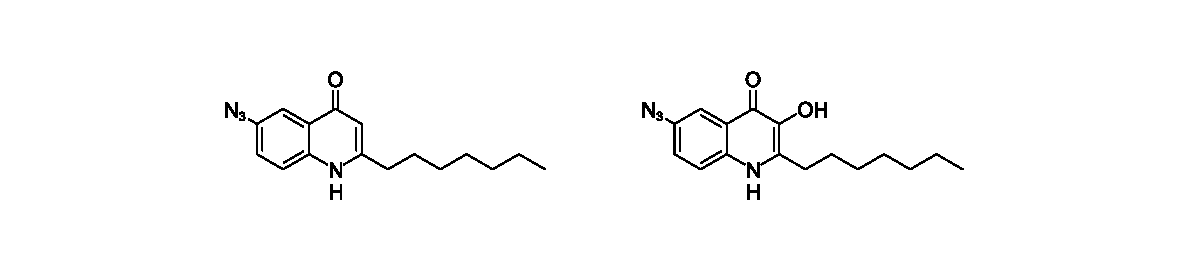
\includegraphics[scale=1]{azHHQPQS}
%		\caption{The HHQ \compound{cmpd:HHQ} and PQS \compound{cmpd:PQS} analogues \compound{cmpd:azHHQ} and \compound{cmpd:azPQS}. \label{fgr:azHHQPQS}}
%	\end{center}
%\end{figure}
%
%\begin{figure}[H]
%	\begin{center}
%		\schemeref[HL2N3]{cmpd:HL2N3}
%		\schemeref[HL4N3]{cmpd:HL4N3}
%		\schemeref[HL6N3]{cmpd:HL6N3}
%		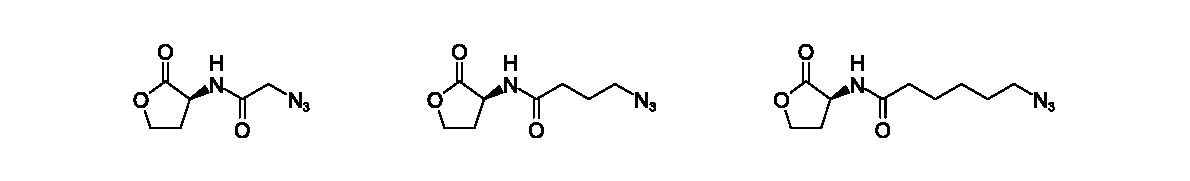
\includegraphics[scale=1]{HL_anas}
%		\caption{The C$_4$-HSL \compound{cmpd:HL4} analogues \compound{cmpd:cmpd:HL2N3}, \compound{cmpd:cmpd:HL4N3} and \compound{cmpd:cmpd:HL6N3}. \label{fig:HL_anas}}
%	\end{center}
%\end{figure}
%
%\subsection{Ciprofloxcin analogues}
%
%Ciprofloxacin \compound{cmpd:cip} (see \ref{fgr:cip_num}) is second-generation fluoroquinolone antibiotic used to treat both Gram-positive and Gram-negative bacterial infections\cite{Oliphant2002}.
%The structure-activity relationships for ciprofloxacin have been investigated \cite{Renau1996} and positions 2 and 7 were found not to cause loss of activity. It was therefore decided that alkyne tails would be added at these positions giving two analogues of ciprofloxacin, \compound{cmpd:hexpipcip} and \compound{cmpd:pipciphex} (see \ref{sch:cip_anas}).
%
%\begin{figure}[H]
%	\begin{center}
%		\schemeref[cip]{cmpd:cip}
%		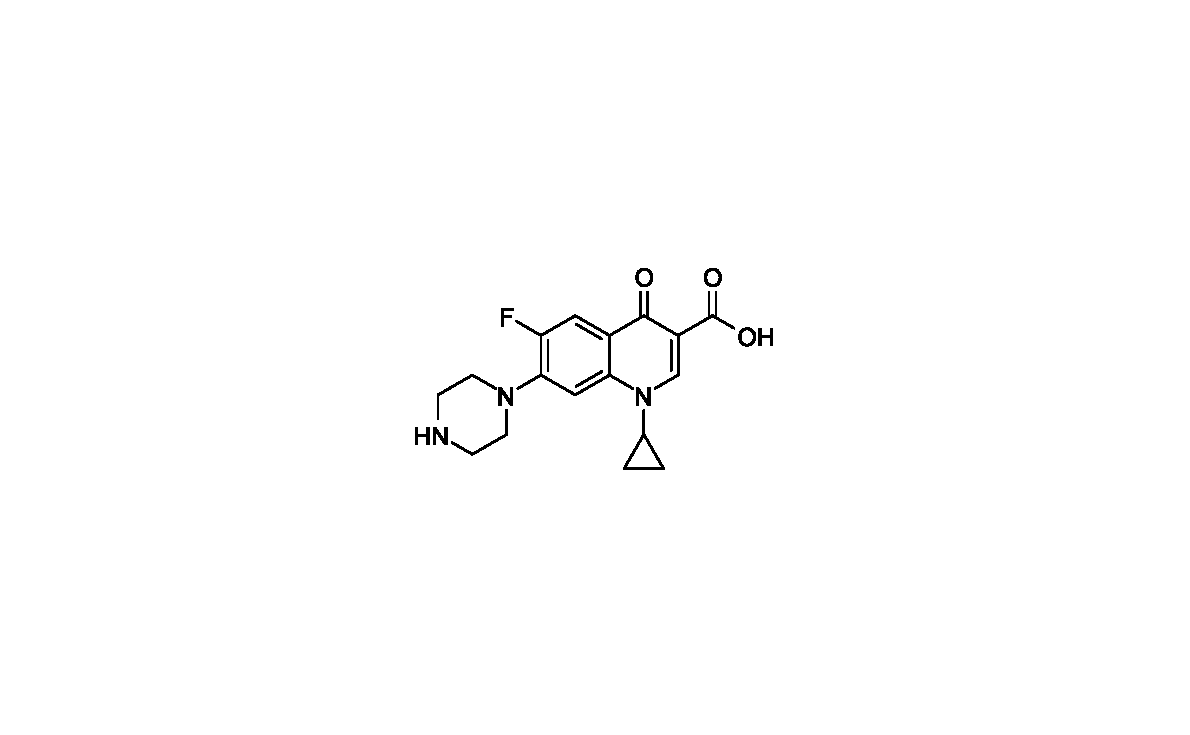
\includegraphics[scale=1]{cip_num}
%		\caption{The atom numbering in ciprofloxacin \compound{cmpd:cip}. \label{fgr:cip_num}}
%	\end{center}
%\end{figure}
%
%\begin{figure}[H]
%	\begin{center}
%		\schemeref[pipciphex]{cmpd:pipciphex}
%		\schemeref[hexpipcip]{cmpd:hexpipcip}
%		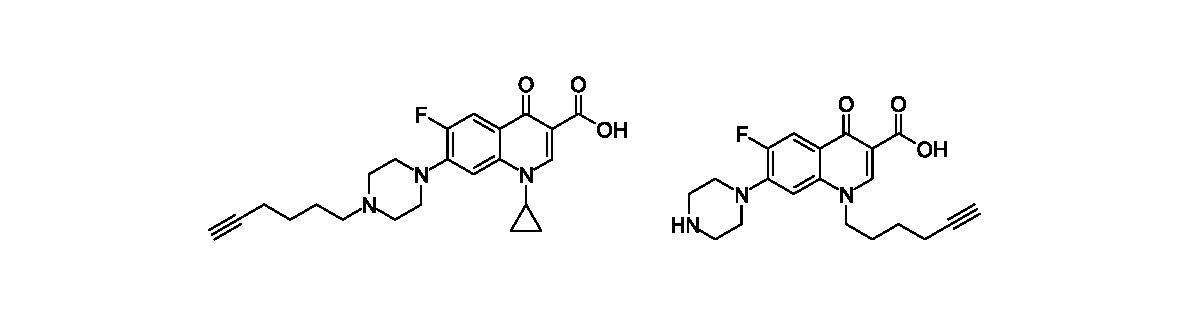
\includegraphics[scale=1]{cip_anas}
%		\caption{The proposed ciprofloxacin analogues \compound{cmpd:hexpipcip} and \compound{cmpd:pipciphex}. \label{sch:cip_anas}}
%	\end{center}
%\end{figure}
%
